\documentclass[12pt,a4paper,openbib,titlepage]{report}
\usepackage{graphicx} % for includegraphics
\usepackage[titletoc]{appendix} % for appendix page
\usepackage{pdfpages} % for including pdf files
\usepackage{setspace} % for \doublespacing
\usepackage{tabularx}
\usepackage{multirow} % for multirow table
\usepackage{tikz} % for drawing
\usepackage{pifont}
\usepackage[backend=biber,style=numeric,citestyle=authortitle-ibid]{biblatex}
\usepackage{amsmath}
\usepackage{amsfonts}
\usepackage{amssymb}
\usepackage[pdftex, plainpages = false, pdfpagelabels, 
pdfpagelayout = OneColumn, % create hyperlinks in citations,figures,tables and refs.
                bookmarks,
                bookmarksopen = true,
                bookmarksnumbered = true,
                linktocpage,
                colorlinks = true,
                linkcolor = black,
                urlcolor  = black,
                citecolor = black,
                anchorcolor = black,
                hyperindex = true,
                ]{hyperref}

\makeatother
\setlength{\oddsidemargin}{0.5cm}
\setlength{\evensidemargin}{0.5cm}
\setlength{\topmargin}{-1.6cm}
\setlength{\leftmargin}{0.5cm}
\setlength{\rightmargin}{0.5cm}
\setlength{\textheight}{24.00cm} 
\setlength{\textwidth}{15.00cm}
\parindent 0pt
\parskip 5pt

\renewcommand{\baselinestretch}{1.25} % for line spacing
\newcolumntype{Y}{>{\centering\arraybackslash}X}
\newcommand{\cmark}{\ding{51}}%
\newcommand{\xmark}{\ding{55}}%

\addbibresource{cite.bib} % include citation file

\begin{document}
	\begin{titlepage}
\begin{center}
		\begin{LARGE}
			\bf{Software Requirements Specification}
		\end{LARGE}
		\vspace*{30pt}
		
		{\large \textbf{Enterprise Resource Planning System(ERP)}}
		\vspace{1.5\baselineskip}
		
		\textit{For}
		\vspace{1.5\baselineskip}
		
		{\large \textbf{Stadia Engineering Works Consultant}}
		\vspace{1.5\baselineskip}	
		
		{\large \textbf{Version 1.0-draft}}
		\vspace{3.5\baselineskip}
		
		
		\vspace{15\baselineskip}
		
		\textit{Prepared by}
		
		\textbf{Adarash Technologies\\
			Addis Ababa, ETHIOPIA\\
			May, 2022 G.C
		}
	
	\end{center}
\pagenumbering{gobble}
\end{titlepage}
	\pagenumbering{roman}
	\addcontentsline{toc}{chapter}{Revision History}



\begin{center}
\section*{Revision History}
\end{center}


\doublespacing
\vspace{1.0cm}
\noindent

\begin{center}
\begin{tabular}{ |c|c|c|c| } 
 \hline
 \textbf{Date} & \textbf{Version} & \textbf{Description} & \textbf{Author} \\ 
 \hline
 May-11-2022 & v1.0-draft & SRS 1.0-draft & Simon Belete \\
  \hline
 May-17-2022 & v1.1-draft & SRS 1.1-draft & Simon Belete \\
 \hline
\end{tabular}
\end{center}
	\addcontentsline{toc}{chapter}{Abstract}
\begin{center}
\section*{ABSTRACT}
\end{center}
\begin{normalsize}
\doublespacing
In today's fast growing of internet users and fast-changing business environment in Ethiopia, it's extremely important to be able to respond to client needs in the most effective and timely manner.Online Shopping is a lifestyle e-commerce web application, which retails various fashion and lifestyle products.The primary goal of an e-commerce site is to sell goods online. This project with developing an e-commerce website and mobile application for Online Product Sale. It provides the user with a catalog of different product available for purchase in the store, viewing various products available enables registered users to purchase desired products process payment by using Cash on Delivery(Pay Later) or Mobile Banking. In order to facilitate online purchase a shopping cart is provided to the user and delivery which is fulfilled by the express system.

Nowadays, many different kinds of delivery companies in Ethiopia transport their own kinds of parcels and offer their own services, which have caused a lot waste of resource. In addition , the volume of parcels in all cities that need to be delivered has been grown dramatically. To cope with these problems, Guya-Express System in the country which can offer service to all kinds of customers in the city including manufactures, department stores, restaurants, individual people and so forth will be designed. This system use combining computer network technology, wireless communication and cloud computing. With this system. the whole package delivery process including classification of packages, vehicle scheduling, path planning, transportation monitoring can be intellectualized as well as managed automatically, and the use of both material resources and manpower resources can be reduced accordingly.

This document will discuss each of the underlying technologies to create and implement and e-commerce and express under the name Guya E-commerce and Guya Express respectively and for architectural implementation we will be using Microservices Architecture.
\end{normalsize}

	\tableofcontents
	\addcontentsline{toc}{chapter}{List of Tables}
	\listoftables
	\addcontentsline{toc}{chapter}{List of Figures}
	\listoffigures
	\addcontentsline{toc}{chapter}{List of Abbreviations}
\begin{center}
\section*{Acronyms and Abbreviations}
\end{center}


\begin{tabular}{p{3cm}p{11cm}}
SRS & Software Requirement Specification \\
ERP & Enterprise Resource Planning \\
LB & Load balancing \\
HQ & Headquarters \\
HR & Human Resources \\
UML & Unified Modeling Language \\
\\
\end{tabular}

	\pagenumbering{arabic}
	\chapter{Introduction}

ERP is one of the most widely implemented business software systems in a wide variety of industries and organizations. ERP is the acronym of Enterprise Resource Planning. ERP is just not only a software. ERP definition refers to both; ERP software and business strategies that implement ERP systems. 

Our Addsoft implementation utilizes Human Resource Management System , Recruitment System, Attendance System, Leave (time off) System, Payroll System , Performance Management (Appraisal) System and Asset Management
to improve the performance of  any organizations for

\begin{itemize}
	\item Resource Planning
	\item Management Control 
	\item Operational Control
\end{itemize}

\section{Open ERP(Odoo)}

Odoo is a comprehensive business applications including Sales, CRM, Project management,
Warehouse management, Manufacturing, Financial management, and Human Resources etc. It is an
all-in-one management software that offers a range of business applications that can form a
complete suite of enterprise management applications targeting companies of all sizes.
Odoo offers a community version and a commercial version. The community version is the open
source free version while the enterprise version are charged at a certain cost and provides more
features and services.
%see appendix I for a complete comparison of the community version and the
%enterprise version. For instance, in Odoo 11, the accounting module which is %essential to an ERP
%system is hidden in the community version, so users will need to enable and %connect the functions
%manually.

Odoo was published first under the name of OpenERP and TinyERP, where ERP stands for
Enterprise Resource Planning. An ERP is a generic software that is flexible to any modification
and customize and fulfills generic needs. Odoo is a modular system where its services are
represented as modules, and the ones that are necessary come installed with the ERP and can be
adapted to the workforce and growth of the company that uses the system. Odoo has a powerful
process engine which allows the allocation of validation modes, tasks and deadlines. According
to the ERP’s official website, Odoo has 5525 module; production management, logistic, human
resources, accounting, management control, payroll, customer relationship management or CRM,
marketing, inventory management, documents management, etc. Odoo is used by many
organizations such as Hyundai, Auchan, Sodexo, Danone, Veolia, and many others.
Odoo is represented in 120 countries by more than 550 partners, and it is used by almost
2,000,000 users.

Odoo is known for a number of features such as:

\begin{itemize}
	\item Social networking
	\item Website creation using CMS
	\item Employee assessment and evaluation
	\item Recruitment process
\end{itemize}

These and other features are exploited by the users to make the management of their business as
organized and smooth as possible.

\subsection{Why choose Odoo}

Why do so many users choose Odoo management software? According to the users’ feedback, these
have been the predominant reasons:

\begin{itemize}
	\item \textbf{Low cost of ownership and no lock-in:} cost of installing, configuring and running an ERP
system is expensive. There is no license fee to run Odoo Community version, so users can
save the cost for implementation and customization. And because it is open source
software, user can download Odoo free of charge, test it and use it.
	\item \textbf{Customizable:} Odoo is flexible to customize to users’ needs. With so many modules, the
user can choose the ones that fits with their business requirements.
	\item \textbf{Comprehensive and modular:} Odoo is an all-in-one business software including CRM,
Website/e-Commerce, billing, accounting, manufacturing, warehouse and project
management, and inventory. The main Odoo components are the OpenObject framework,
about 30 core modules and more than 3000 community modules.
	\item \textbf{Updated technology:} Odoo is based on a technology stack which is modern and up-to-date.
And with its open source community, it is actively maintained by a large base of developers
to meet customer’s needs and provide new applications.
\end{itemize}

\section{Scope}

\begin{description}
	\item[Human Resources:] Human Resources Module
	\begin{itemize}
		\item Create and manage employee profile
 		\item Create and manage employee profile
 		\item Create and manage Departmental hierarchy
 		\item Create and manage contracts
 		\item Employee dashboard
 		\item Import and export to Excel
 	\end{itemize}
 	
 	\item[Recruitment:] Recruitment Module
	\begin{itemize}
		\item Create job position
		\item Publish vacancies
		\item Review applications
		\item Manage departments
 	\end{itemize}
 	
 	\item[Attendance:] Attendance Module
	\begin{itemize}
		\item Tap in and tap out
		\item Reporting Dashboard
		\item Import and export to Excel
		\item Integrate with Payroll
 	\end{itemize}
 	
 	\item[Leave (time off):] Leave (time off) Module
	\begin{itemize}
		\item Annual and other leave type
		\item Maintain Leave quota
		\item Employee self service
		\item Manager approval
		\item Integrate with Payroll
 	\end{itemize}
 	
 	\item[Payroll:] Payroll Module
	\begin{itemize}
		\item Salary structure
		\item Setup payroll component 
		\item Contract Management
		\item Reporting Dashboard 
		\item Print pay slip and email pay slip
		\item Protect pay slip file with password
		\item Integrate with another modules
 	\end{itemize}
 	
 	\item[Performance Management (Appraisal):] Performance Management (Appraisal) Module
	\begin{itemize}
		\item Create and manage Employee appraisal 
		\item Set evaluation scale
		\item Create goal
		\item Sort appraisal
		\item Generate report
 	\end{itemize}
 	
 	\item[Asset Management:] Asset Management Module
	\begin{itemize}
		\item Maintain asset record 
		\item Assign asset to employee
		\item Depreciation
		\item Generate report
 	\end{itemize}
\end{description}


\section{System Requirements}

\subsection{Hardware Requirements}

Odoo is an undemanding system. For 5-employee companies, a 2 CPU 2 RAM server would be enough (recommended 8 RAM), raising to 4 CPU 8 RAM for 20 employees. We would recommend splitting application and database servers for 90 employees. Load balancing (LB) of application server would be needed for a company of 250+ employees.

\begin{figure}[!ht]
\center
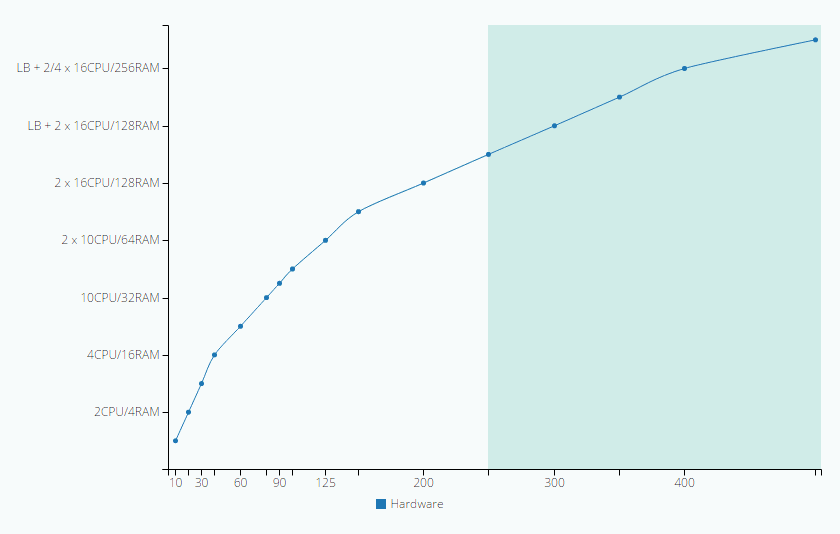
\includegraphics[width=15cm,keepaspectratio]{images/odoo_server_requirments_graph.png}
\caption{Odoo server requirements}
%\source{Source: Michael Aldrich Archive}
\label{pre-production-fig}
\end{figure}

\subsection{Software Requirements}

\begin{description}
	\item[Postgresql v14.0:] Is a powerful, open source object-relational database
	\item[Odoo community v14:] Is a suite of business management software tools
	\item[Docker:] Is a set of platform as a service products that use OS-level virtualization to deliver software in packages called containers
	\item[Docker compose:] Is a tool for defining and running multi-container Docker applications
	\item[Python v3.7] Is a high-level, interpreted, general-purpose programming language.
\end{description}









	\chapter{System Analysis}

\subsection{System Requirement Specification}

General structure of a user story described in this document: 
\\ \\
\begin{normalsize}
\textbf{\{User story name\}}: As a \{role\}, I want \{goal\}, so that \{benefit\} (\{priority\}).
\end{normalsize}

\subsection{Functional Requirements}
The following sections describe the data required and the functional requirements that shall be performed in the new ERP System for both the HQ and field-based staffs.  These functional requirements include the on-going System maintenance and the creation and management reports for all areas.

\begin{itemize}
	\item The System shall have a common database core which allows integration of data and transactions between all financial, operational, production, and customer service functions within the ERP System.
	\item The System shall have a graphic user interface (GUI) implemented  as a Web-based interface
	\item The System shall be able to export selected records into either pdf or table file format
	\item The System shall have administrator ERP System and user security functionality to include:
		\begin{itemize}
			\item Setting Up a New User
			\item Updating an Existing User
			\item Restricting User Access to Certain Roles
		\end{itemize}
	\item The System shall have the ability for generated reports to be savable and exportable to numerous devices and mediums including printers
	\item The System shall produce Fixed Asset Depreciation Schedules
\end{itemize}

\subsection{Non-functional Requirements}

\paragraph{Reliability}
Reliability is the probability that the System will be able to process work correctly and completely without being aborted.
\\
The proposed ERP System has varying degrees of impact on areas of Stadia should parts of the System fail.
If the Core Systems functional areas of the System fail (becomes unusable) for a period of time the impact on Stadia would be as follows:

\begin{center}
\begin{table}[!hb]
\begin{tabular}{ | m{10em} | m{25em}| } 
  \hline
  \textbf{Length of Time of Outage} & \textbf{Impact to Stadia} \\ 
  \hline
   One Hour & Some Impact to {{TODO}} \\ 
   \hline
   One Day & Medium to Large Impact {{TODO}} \\
   \hline
   One Week & Very Large to Catastrophic Impact. \\
  \hline
\end{tabular}
\caption{Impact of reliablity on Stadia}
\end{table}
\end{center}

The minimum acceptable level of reliability for the core system Reporting aspect of the System would be no more than five (5) days (one work week).

\paragraph{Recoverability}
Recoverability is the ability to restore function and data in the event of a failure.

\begin{itemize}
	\item In the event the ERP application is completely unavailable to users (down) because of a System failure, it should be restored within 2 hours after the failure is detected.  This timeframe assumes that a locally controllable event (such as a hardware issue) has caused the outage.  If the application software is at issue and requires Contractor intervention, then the expected restoration time shall follow expected levels that shall be stated in the Service Level Agreement. 
	\item In the event that the operational database is corrupted, the database must be capable of being restored to its condition no more than 2 hours before the corruption occurred and must be restored to its most recent point in time prior to the corruption (1 day before). (Once a Contractor is selected a final data recovery strategy shall be determined).
\end{itemize}

The core system will perform periodic backups of all databases and will store these backups off-site.  At a minimum daily incremental changes to the database shall be captured and stored and on a weekly basis and a full database backup should be performed.  Daily backups shall be retained for at least six weeks (approximately one monthly close cycle) and weekly backups should be retained for at least fourteen weeks (one quarterly close cycle).  

In the event that the entire data center is destroyed, the following steps shall be required:
\begin{itemize}
	\item New Application and Database Servers would need to be located and installed
	\item Operating Systems shall need to be set up on the Servers(i.e Linux Server)
	\item Applications the ERP core System (Odoo) shall need to be installed on the Servers
	\item The last off-site back up of the ERP application database shall be restored to the Servers
\end{itemize}

\paragraph{System Availability}
System availability is the time when the application must be available for use. Required System availability is used in determining when maintenance may be performed.

The System must be available from 2:00 AM – 11:00 PM GMT+3 Monday – Saturday (National Holiday and Service Reduction Days not included).  Any scheduled down time for maintenance shall be not be scheduled around these core hours.

\paragraph{Fault Tolerance}
Not Applicable refer to Odoo Guideline

\paragraph{Performance}
The current preference is that accessing any transactional screen and updating data fields should take no more than 3 seconds.

System performance should be measured using up to 10 to 300 concurrent users(based on Stadia's number of employee)

\paragraph{Capacity}
The ERP System shall have the capacity to handle the types of volumes described below:
\begin{itemize}
	\item {TODO} number of employee creation per month
	\item {TODO} reports per month
\end{itemize}

\paragraph{Data Mapping and Conversion}
The following tables describe the data in the current system. he file structures and data in the current system are housed in Postgressql tables but are not truly relational in design.

\begin{itemize}
	\item A = Alphanumeric
	\item D = Date (MM/DD/YYYY)
	\item N = Numeric
\end{itemize}

\begin{center}
\begin{table}[!hb]
\begin{tabular}{|c|c|c|c|c| } 
  \hline
  \textbf{Ref} & \textbf{Description} & \textbf{Field Type} & \textbf{Note} & \textbf{Field Length (Bytes)} \\ 
  \hline
  1 & Badge ID & A & Generated Badge Number ID & 6 \\ 
  \hline
\end{tabular}
\caption{Datat mapping and conversion}
\end{table}
\end{center}


\paragraph{Design, Testing, Implementation, and Acceptance}
The Contractor/Provider shall be responsible for:

\begin{itemize}
	\item The design and configuration of the new ERP System based on Stadia business requirements.
	\item Installation of the ERP System in a test environment
	\item Loading the test database with sufficient data to perform the required User Acceptance Testing. This task shall be on-going until successful completion of the User Acceptance Testing. Both Stadia and Adarash will provide the User Acceptance Testing Matrix.
	\item Setup of the software and activation of the modules.
	\item Setup of the master files and tables and work with Stadia's staff to verify the data.
	\item Implementation of the ERP System into the final production environment.
	\item 
\end{itemize}

\paragraph{Training and Documentation}
The Contractor/Provider shall be responsible for:

\begin{itemize}
	\item Training of end users and technical staff to support to the ERP System to include:
		\begin{itemize}
			\item General Manger
			\item System Admin(IT staff)
			\item Clerks
			\item Department heads
		\end{itemize}
	\item Retraining for personnel as needed or requested by management
	\item Creating a learning team of "super users"(System Admins or IT staff) who can support others in all basic and some advanced functions
	\item Providing and/or creating training materials and technical documentation of the ERP System to include Quick Reference guides and an inmate self-learning module.
\end{itemize}

\section{System Requirement Analysis}

\subsection{Actor and Use Case Identification}
A use case diagram is a graphic depiction of the interactions among the elements of a system. A use case is a methodology used in the system analysis to identify, clarify, and organize system requirements in this context, the term \"system" refers to something being developed or operated such as a mail-order product sales and service website. Use case diagram are employed in UML (Unified Modeling Language). A standard notation for the modeling of real-world object and systems. System objectives can include planning overall requirements validating a hardware design, testing and debugging a software product under development, creating an online help reference, or performing a consumer-service oriented task. For example, use case in a product sales environment would include item ordering, catalog updating payment processing, and customer relations. A use case diagram contains four components.

\begin{figure}[!h]
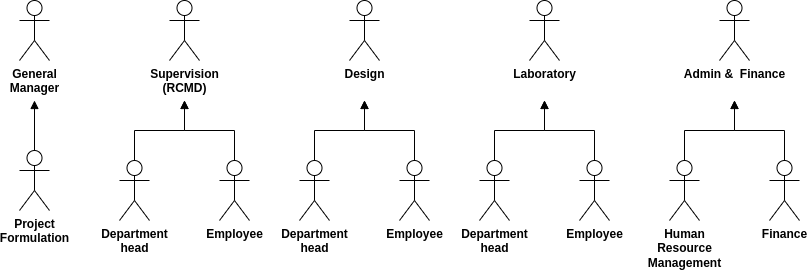
\includegraphics[width=13cm, keepaspectratio]{usecases/actors.png}
\label{shop_actors}
\caption{Actors involved }
\end{figure}

\subsection{Use Case Diagram}

Use case diagrams are used during the analysis
process to find system requirements and to design
system functionality. In this study use case
diagrams are used to describe the access rights of
each actor. Administrator Actors generally have a
function to manage users such as creating accounts
and setting access rights.

\subsubsection{Use Case Diagram And Description}
Website security requirements mandate separation of administrative interface from common functions provided to users. This segregation, for example, is strongly recommended by ISO 17799.

System should have separate application for administrators and for common users. It is recommended by OWASP Guide 2.0\footcite{https://www.owasp.org} that website administration application should not be accessible from  the internet without going through some management networks eg. via a strongly authenticated VPN or from a trusted network operation center.

Except for administrators, some part of the administrative interfaces should be also available to the Help desk staff (Customer Service) and some staffs, as they need to be able to assist customers having issues while using the customer oriented website.

Top level use case diagram below shows some administrative functions that administration website could provide.

%\paragraph{Top Level Use Case Diagram}
\begin{figure}[!hb]
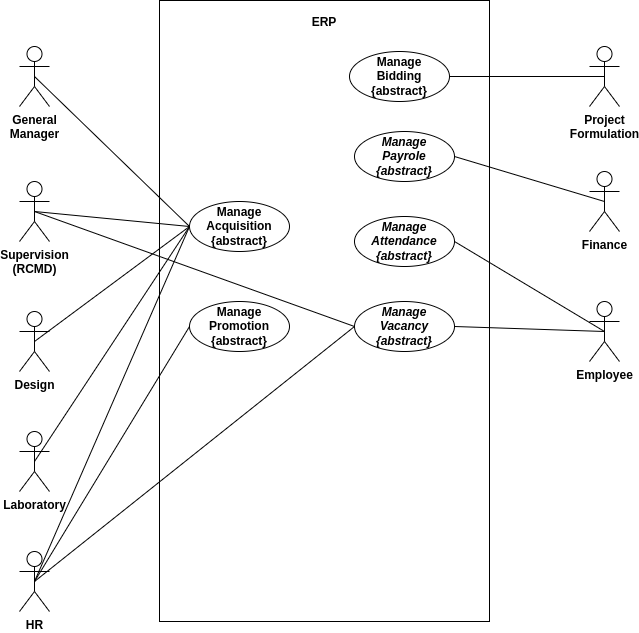
\includegraphics[width=15cm,keepaspectratio]{usecases/top_level_usecase.drawio.png}
\caption{Top level use case diagram}
\end{figure}

%################################# Acquisition #############################
\begin{figure}[!ht]
\centering
%\vspace*{-8cm}
%\hspace*{-3cm}
%\noindent
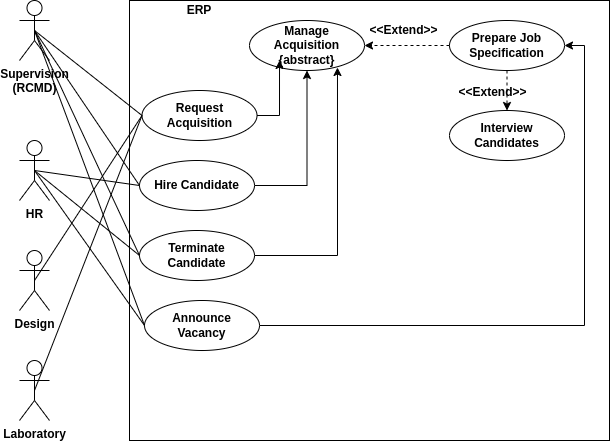
\includegraphics[width=10cm,keepaspectratio]{usecases/acquisition_usecase.drawio.png}
\caption{Manage Acquisition use case diagram }
\end{figure}
%################################# End Of Acquisition############################# 

%################################# Recruitment #############################
\begin{figure}[!ht]
\centering
%\vspace*{-8cm}
%\hspace*{-3cm}
%\noindent
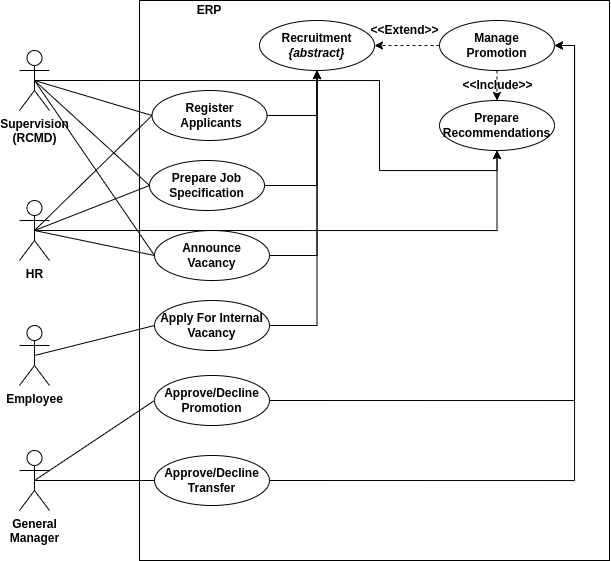
\includegraphics[width=15cm,keepaspectratio]{usecases/recruitment.drawio.png}
\caption{Manage Acquisition use case diagram }
\end{figure}
%################################# End Of Recruitment ############################# 


%################################# Loan #############################
\begin{figure}[!ht]
\centering
%\vspace*{-8cm}
%\hspace*{-3cm}
%\noindent
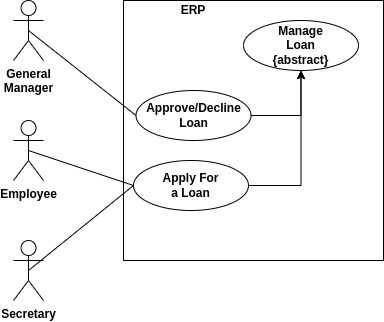
\includegraphics[width=10cm,keepaspectratio]{usecases/loan.drawio.png}
\caption{Manage Acquisition use case diagram }
\end{figure}
%################################# End Of Loan ############################# 

%################################# Payroll #############################
\begin{figure}[!ht]
\centering
%\vspace*{-8cm}
%\hspace*{-3cm}
%\noindent
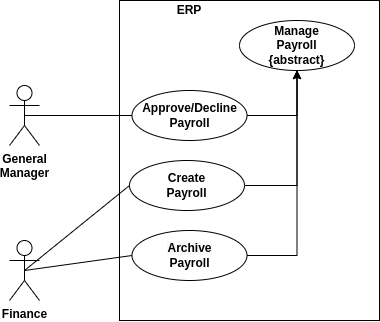
\includegraphics[width=10cm,keepaspectratio]{usecases/payroll.drawio.png}
\caption{Manage Acquisition use case diagram }
\end{figure}
%################################# End Of Payroll ############################# 


%################################# appraisal #############################
\begin{figure}[!ht]
\centering
%\vspace*{-8cm}
%\hspace*{-3cm}
%\noindent
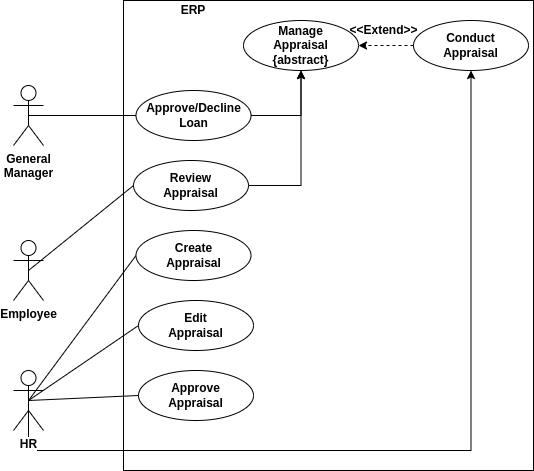
\includegraphics[width=10cm,keepaspectratio]{usecases/appraisal.drawio.png}
\caption{Manage Acquisition use case diagram }
\end{figure}
%################################# End Of Attendacne ############################# 

\begin{figure}[!ht]
\centering
%\vspace*{-8cm}
%\hspace*{-3cm}
%\noindent
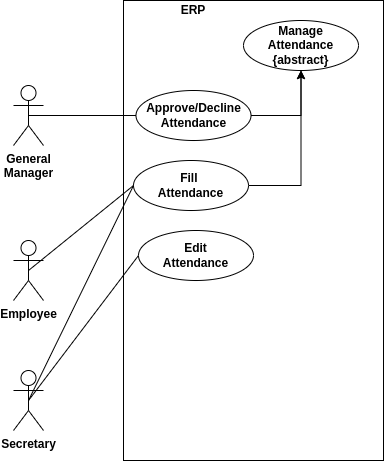
\includegraphics[width=10cm,keepaspectratio]{usecases/attendance.drawio.png}
\caption{Manage Acquisition use case diagram }
\end{figure}
%################################# End Of Attendacne ############################# 

\begin{figure}[!ht]
\centering
%\vspace*{-8cm}
%\hspace*{-3cm}
%\noindent
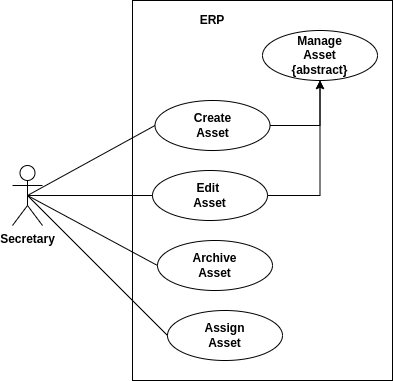
\includegraphics[width=10cm,keepaspectratio]{usecases/asset.drawio.png}
\caption{Manage Acquisition use case diagram }
\end{figure}
%################################# End Of Asset ############################# 



%\subsubsection{Administrator Use Case Diagram}

%\subsubsection{Manager Use Case Diagram}

%\subsubsection{HR Use Case Diagram}

%\subsection{Activity Diagram}

%\subsubsection{Recruitment Module Activity Diagram}

%\subsubsection{Human Resources Activity Diagram}

%\subsubsection{Attendance Activity Diagram}

%\subsubsection{Leave (time off) Activity Diagram}

%\subsubsection{Payroll Activity Diagram}

%\subsubsection{Performance Management (Appraisal) Activity Diagram}

%\subsubsection{Asset Management Activity Diagram}


\subsection{User Access Rights}

\hspace{-2cm}
\begin{tabularx}{540pt}{|X|c|c|c|c|c|c|c|p{3cm}|}

%{|*{9}{Y|}}

\hline

\textbf{No} & \textbf{User} & \textbf{Acess Level} & \textbf{Object} & \multicolumn{4}{c|}{\textbf{Acess Right}} & \textbf{Information} \\
\cline{5-8} & &  &  & Read & Write & Create & Delete & \\

\hline

\multirow{1}{*}{1} & \multirow{1}{*}{Administrator} & \multirow{1}{*}{Administration} & ALL & \cmark & \cmark & \cmark & \cmark & Top Level \\

\hline

\multirow{2}{*}{2} & \multirow{2}{*}{System Admin} & \multirow{2}{*}{System Admin} & 
User & \cmark & \cmark & \cmark & \xmark & Second level below Administrator \\
\cline{4-8} & & & 
Acess Right 2 & \xmark & \xmark & \xmark & \xmark & \\

\hline

\multirow{2}{*}{3} & \multirow{2}{*}{Manager} & \multirow{2}{*}{Manger} & 
Attendance & \cmark & \cmark & \xmark & \xmark & Manager \\
\cline{4-8} & & & 
Acess Right 2 & \xmark & \xmark & \xmark & \xmark & \\

\hline

\end{tabularx}
\hspace*{-1cm}


	\chapter{System Design}
	\chapter{Implementation}
	\chapter{Testing}
	\appendix
\appendixpage

\begin{appendices}

\end{appendices}
	\addcontentsline{toc}{chapter}{Reference}
	\nocite{*}
	\printbibliography[title={References}]
\end{document}